\documentclass[10pt]{article}
\usepackage[top=1in, bottom=1.25in, left=1in, right=1in]{geometry}
\usepackage{amsmath}
\usepackage{amssymb}
\usepackage{enumitem}
\usepackage{graphicx}


\usepackage{fancyhdr}
\pagestyle{fancy}
\lhead{MATH7241: Project Report}
\rhead{David Zhao\\Benjamin Quiring\\\today}
\setlength{\headheight}{40pt}

\newcommand{\solution}{\textbf{Solution. }}
\newcommand{\deff}{\underline{Def. }}
\newcommand{\thm}{\underline{Theorem. }}
\newcommand{\lemma}{\underline{Lemma. }}
\newcommand{\corollary}{\underline{Corollary. }}
\newcommand{\proof}{\emph{Proof }}

%\newenvironment{proof}{\par\noindent{\it Proof.}\hspace*{1em}}{$\Box$\bigskip}

\setlength{\parindent}{0em}
\setlength{\parskip}{0.5em}
\begin{document}
\section{Data}
We downloaded a history of terminal commands for a UNIX computer from Perdue
back in 1998. A sample of the data looked like:
\begin{verbatim}
cd
<1>
ll
vi
<1>
ll
emacs
\end{verbatim}

Where a \texttt{<\#>} represents the number of arguments given to a command.
This was done to preserve the user's privacy. We cleaned the data as follows:
\begin{enumerate}
  \item We combined a command with the number of arguments passed with it. For
    example \texttt{cd<1>} is different from \texttt{cd} which is also different
    from \texttt{cd<2>}.
  \item We ignored operators like \texttt{; , -, |} and didn't consider them
    commands.
  \item We ignored the \texttt{**SOF**} and \texttt{**EOF**} commands because
    they were added and not actually typed by the user.
\end{enumerate}
After cleaning up the data as described above, we noticed that there were over
$700$ unique commands. We chose the $28$ most common occuring commands to be the
states in our Markov chain and proceeded to further filter the data by deleting
commands that are not the $28$ most common. The resulting dataset contained only
the top $28$. There were over twenty thousand time steps in the filtered data.
We plotted the entire time series and the first 250 steps.

\begin{figure}[ht]
  \centering
  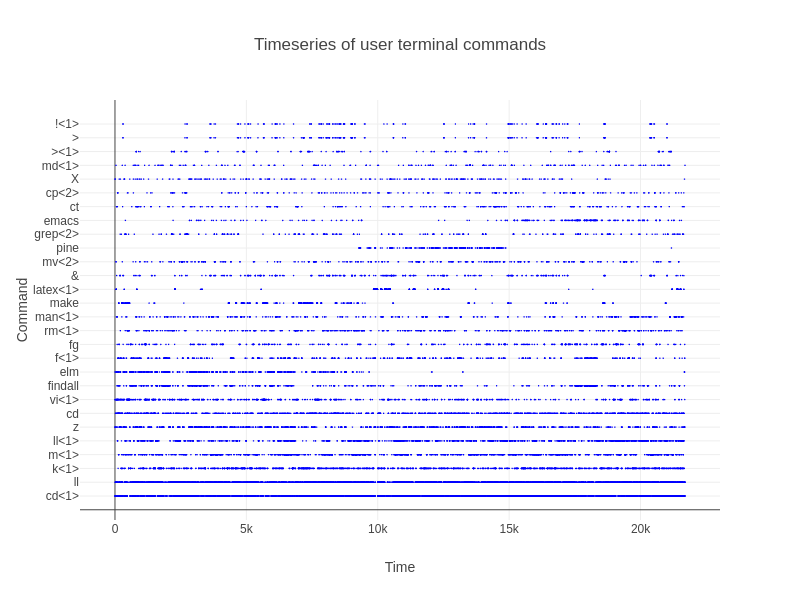
\includegraphics[scale=.65]{../pictures/complete-emperical-timeseries.png}
\end{figure}

\begin{figure}[ht]
  \centering
  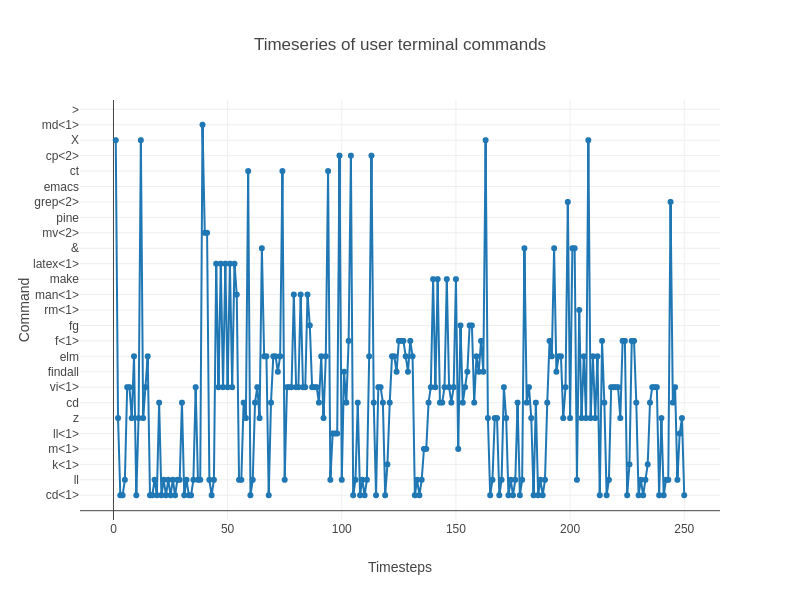
\includegraphics[scale=.65]{../pictures/250-emperical-timesteps.png}
\end{figure}

We calculated the occupation frequencies of the emperical data and graphed the
distribution.

\begin{figure}[ht]
  \centering
  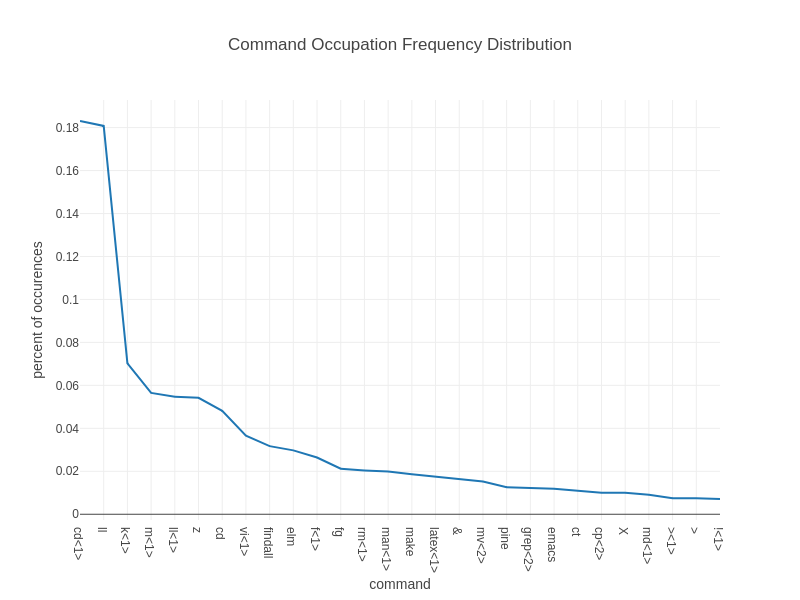
\includegraphics[scale=.65]{../pictures/emperical-occ-freq-dist.png}
\end{figure}

Even though the data is from 1998 the top 5 commands seem reasonable given our
own experience using UNIX based operating systems. The majority of the time a
user will be navigating their computer's file directory with commands like
\texttt{cd} and \texttt{ll}

Next we computed the transition matrix by counting the number of times the chain
went from state $i$ to state $j$ followed by dividing each count $P_{ij}$ by the
number of times we moved out of state $i$.

The transition matrix, plotted as a heatmap looked like:

\begin{figure}[ht]
  \centering
  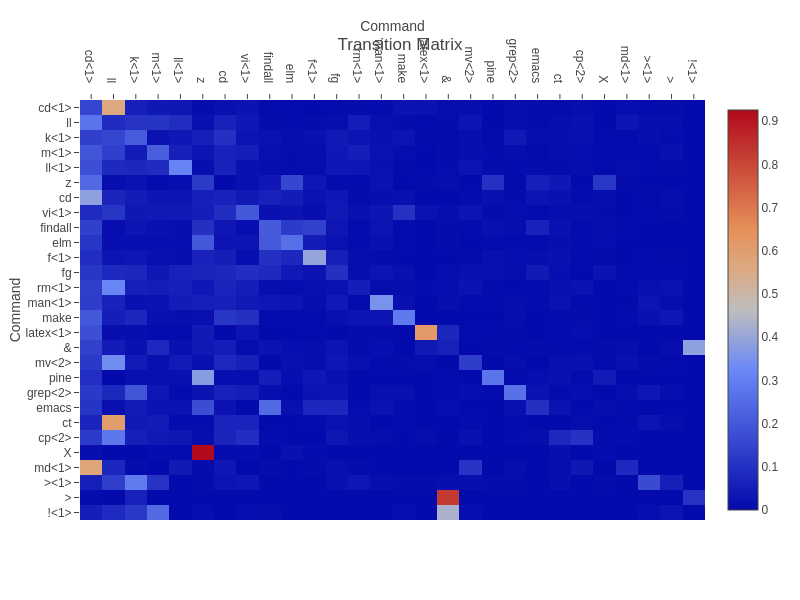
\includegraphics[scale=.65]{../pictures/transition-matrix-heatmap.png}
\end{figure}

We raised the transition matrix to the power $1000$ to compute the stationary
distribution. We argue that the chain is irreducible because the data tracks the
user's usage of the UNIX machine over two years. This means that there are many
instances of logging in and out of the machine, which is done with the same set
of commands every time (\texttt{rlogin} and \texttt{exit}). So the only instance
where a state $i$ is unreachable from $j$ is if the user types a command and
then doesn't proceed to logoff or doesn't proceed to log on. Both cases are
impossible because a command isn't tracked until the user has logged on and
since we're tracking the $28$ most common commands there is no way that one of
these commands are used so frequently while the user never exit afterwrods.
Therefore, since the chain always visits the state \texttt{exit} every state can
reach \texttt{exit} and as a result every state can reach every other state via
the \texttt{exit} state.

Therefore, when we plot the stationary distribution
against the occupation frequency distribution, it is no surprise that the
distributions are identical.

\begin{figure}[ht]
  \centering
  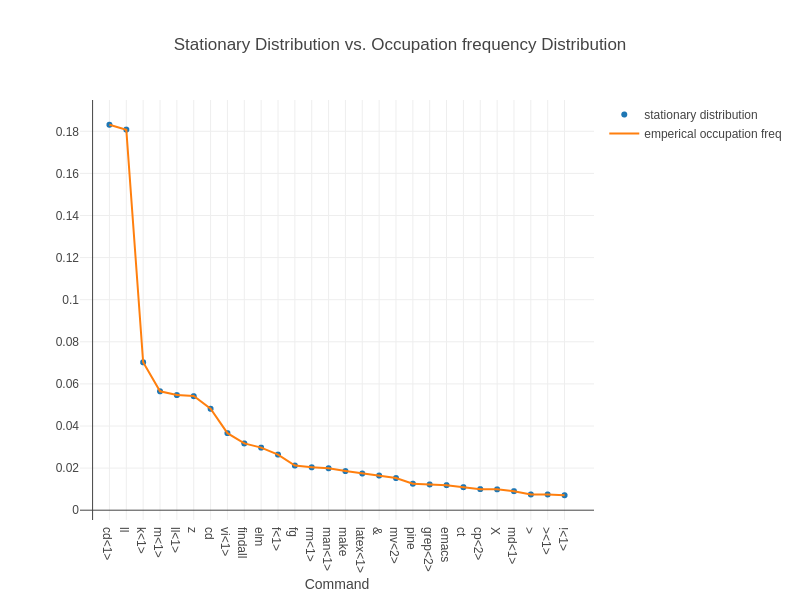
\includegraphics[scale=.65]{../pictures/stat-dist-and-emperical-occ-freq-dist.png}
\end{figure}

Finally we simluated the chain for $250$ time steps. We assumed that the initial
distribution was uniform over all the states.

\begin{figure}[ht]
  \centering
  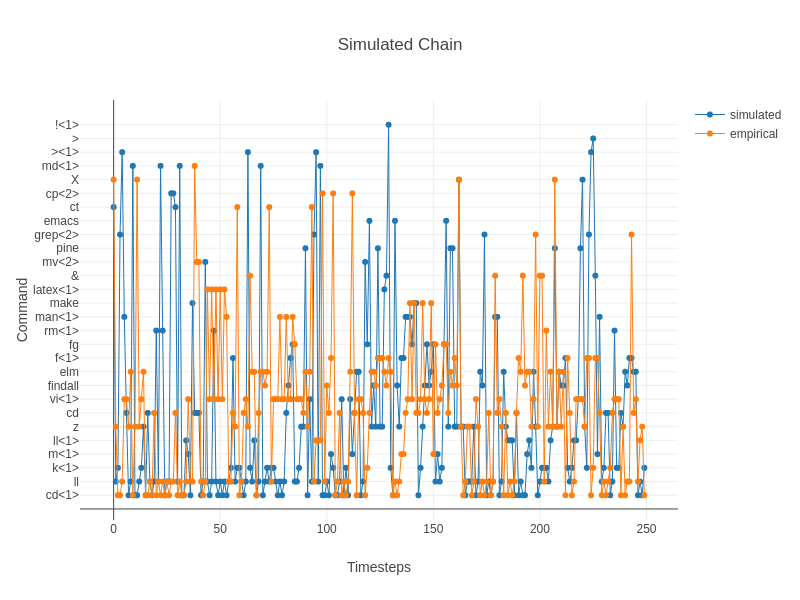
\includegraphics[scale=.65]{../pictures/simul-chain-vs-emperical-chain.png}
\end{figure}

Finally we investigated the mixing time of the chain. We did this by, at each
time step, computing the occupation frequency of the chain from the first to the
last time step. At each step we calculate the occupational frequency of the
states seen so far and subtracted this distribution with the calculated
stationary distribution. We then plotted the l2 norm of the difference.

\begin{figure}[ht]
  \centering
  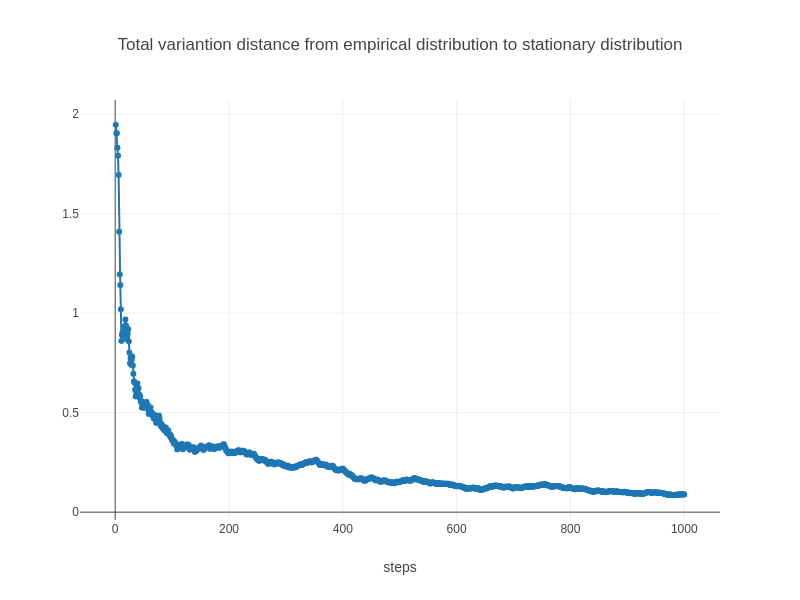
\includegraphics[scale=.65]{../pictures/mixing-time-analysis.png}
\end{figure}

\end{document}

